\documentclass{/home/janmebows/Documents/LatexTemplates/myassignment}

\title{Topic C Assignment 1}

\begin{document}

\maketitle
\begin{enumerate}
    \item 
    \begin{enumerate}
        \item There are $2$ non-zero roots to the equation. This is shown in Figure~\ref{fig::tanhx}.\\
        \begin{figure}
            \centering
            \label{fig::tanhx}
            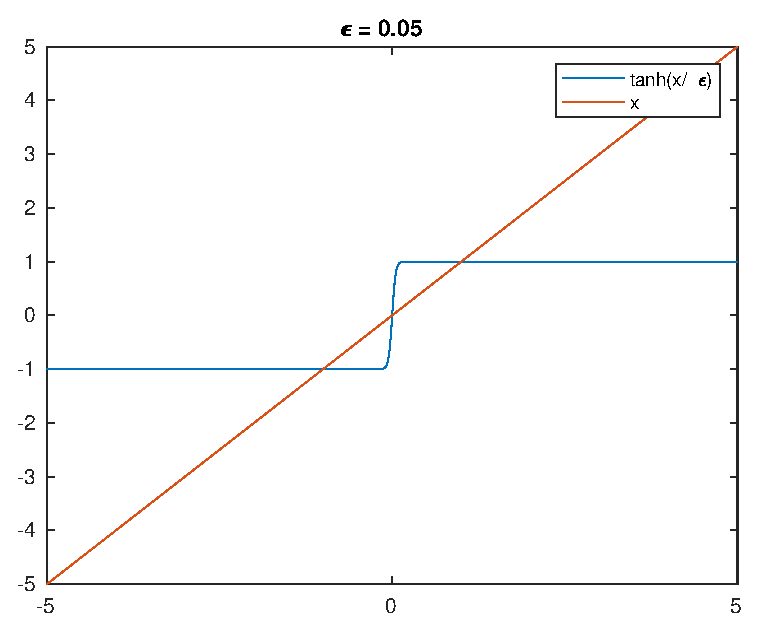
\includegraphics{TopicCA1Q1a.eps}
            \caption{plot of $\tanh(x/\epsilon)$ and $x$ for $\epsilon=0.0001$}
        \end{figure}
        \item Use $x = \pm 1 + S$ where $S\ll 1$, and $tanh(x) = \frac{e^{2x}-1}{e^{2x}+1}$\\
        Note that $\tanh(x)$ is an odd function, so the solution around $x=-1$ will be the negative of the solution around $x =1$.\\

        Take the taylor series of $\tanh(x/\epsilon)$ about $x = \pm 1$
        \[\tanh(x/\epsilon) = \tanh(\pm \frac1\epsilon) + \sech^2(\frac1\epsilon)\]

        So $x = \tanh(x/\epsilon)$
        \begin{align*}
            x =& \tanh(x/\epsilon)\\
            x=& \frac{2}{1 + e^{-2x/\epsilon}} - 1\\
            x=& 2 - 2e^{-2x/\epsilon} + 2e^{-4x/\epsilon} - o(e^{-4/\epsilon})-1\\
            x=& 1 - 2e^{-2x/\epsilon} + 2e^{-4x/\epsilon} - o(e^{-4/\epsilon})\\
        \end{align*}
        Since $x = 1 + S + S_2$ Where $S \ll 1$ and $S_2 \ll S$, we get
        \begin{align*}
            x=& 1 - 2e^{-2x/\epsilon} + 2e^{-4x/\epsilon} - o(e^{-4/\epsilon})\\
            1 + S +S_2 &=1 - 2e^{-2(1+S+S_2)/\epsilon} + 2e^{-4(1+S+S_2)/\epsilon} - o(e^{-4/\epsilon})\\
            S+S_2 &=  -2e^{-2(1+S+S_2)/\epsilon} + 2e^{-4(1+S+S_2)/\epsilon} - o(e^{-4/\epsilon})\\
        \end{align*}
        Since $S\ll 1$ and $S_2 \ll S$ $e^{-(1+S+S_2)/\epsilon} \approx e^{-1/\epsilon}$. Giving
        \begin{align*}
            S+S_2 &=  -2e^{-2(1+S+S_2)/\epsilon} + 2e^{-4(1+S+S_2)/\epsilon} - o(e^{-4/\epsilon})\\
            S+S_2 &=  -2e^{-2/\epsilon} + 2e^{-4/\epsilon} - o(e^{-4/\epsilon})\\
            \implies S &= -2e^{2/\epsilon}\\
            \implies S_2 &= 2e^{-4/\epsilon}
        \end{align*}
        Which then gives:
        \[x_+ = 1 -2e^{-2/\epsilon} + 2e^{-4/\epsilon} - \bigo(e^{-6/\epsilon})\]
        And 
        \[x_- = -(1 -2e^{-2/\epsilon} + 2e^{-4/\epsilon} - \bigo(e^{-6/\epsilon}))\]

        \item Figure~\ref{fig:2c} compares the 3 term asymptotic solution to the numerically obtained solution for $x=\tanh(x/\epsilon)$. As $\epsilon\to 0$ it is clear that the asymptotic solution quickly approaches the numerical solution
            \begin{figure}
                \centering
                \label{fig:2c}
                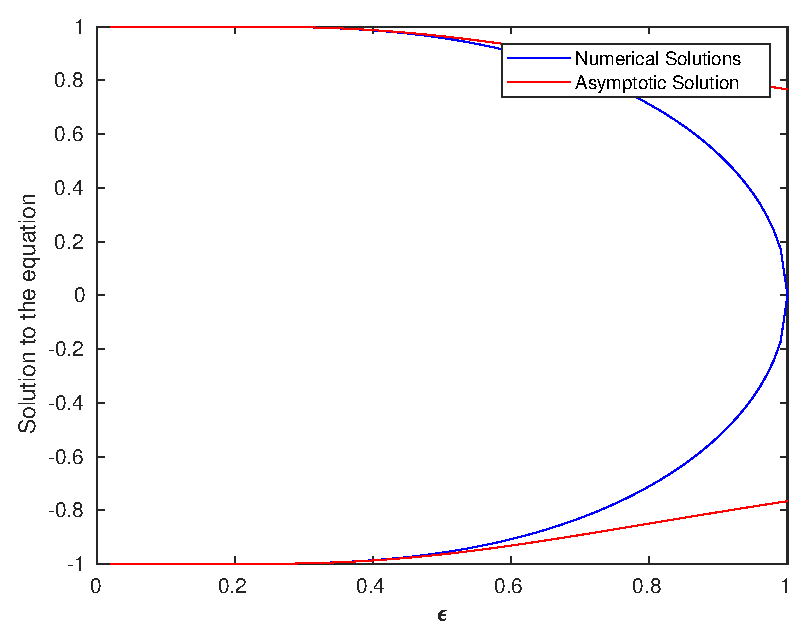
\includegraphics{TopicCA1Q1c}
                \caption{Comparison of asymptotic solution to numerical Solution of $x = \tanh(x/\epsilon)$}
            \end{figure}
    \end{enumerate}
\clearpage
%%%

%%Question 2
%%%  
   \item 
    \begin{enumerate}
        \item If we rewrite the differential equation in standard form, we get:
        \[y'' - \frac{1}{x^2} y' + \frac1{4x^4} y = 0\]
        From this, $x=0$ is an irregular singular point since $x \frac{-1}{x^2}= -\frac{1}{x} \to -\infty, \ as \ x\to 0$. While all other values of $x$ are ordinary points.
        
        \item Since $x=0$ is an irregular singular point, use  $y = e^{S(x)} := e^{S}$:
        \begin{align*}
            y' &= S' e^{S} \\
            y'' &= S'' e^{S} + (S')^2 e^{S}
        \end{align*}
        \begin{align*}
            x^4 (S'' e^{S} + (S')^2 e^{S}) - x^2 (S' e^{S}) + \frac14 e^{S} = 0\\
            S'' + (S')^2 - x^{-2} (S') + \frac1{4x^4} = 0\\
        \end{align*}
        Now for asymptotic balance:
        \begin{itemize}
            \item $S'' \sim -(S')^2$ as $x\to 0$, assuming $x^{-2}(S') , \frac1{4x^4} \ll S'', -(S')^2$
            \begin{align*}
                &\frac{S'}{S^2} \sim -1\\
                &S' \sim \frac{1}{x+a}\\
                \implies &-(S')^2 \sim -\frac{1}{(x+a)^2},\, x\to 0
            \end{align*}
            Which is a \textbf{contradiction} as $\frac{1}{4x^{4}} \not\ll -(S')^2$ as $x\to 0$ and likewise $x^{-2} S' \not \ll -(S')^2$.
            
            
            \item $S'' \sim x^{-2} (S')$ as $x\to 0$, neglecting $-(S')^2$ and $\frac{1}{4x^4}$
            \begin{align*}
                \frac{S''}{S'} \sim x^{-2}\\
                \log S' \sim \frac{-1}{x} + b\\
                S' \sim c e^{-1/x}\\
                \implies -(S')^2 \sim -c e^{-2/x}
            \end{align*}
            Which is a \textbf{contradiction}, as $\frac1{4x^4} \gg e^{-2/x}$ as $x\to0$. And $-(S')^2 \not \ll S''$
            
            \item $S'' \sim -\frac{1}{4x^4}$ as $x\to 0$, neglect $-(S')^2$ and $x^{-2}(S')$
            \begin{align*}
                S' \sim \frac{1}{12x^3}\\
                -(S')^2 \sim \frac{-1}{144 x^{6}}
            \end{align*}
            \textbf{Contradiction} since we have neglected $-(S')^2$ but $S'' \ll -(S')^2 $, as $x\to 0$. And similarly $x^{-2} S' \gg (\frac1{4x^4})$
            
            
            \item $(S')^2 \sim x^{-2}(S')$ as $x\to 0$, neglecting $\frac1{4x^4}$ and $S''$
            \begin{align*}
                S' \sim x^{-2}\\
                \implies (S')^2 \sim x^{-2}(S') \sim \frac{1}{x^4}\\
                S'' \sim \frac{-1}{2x}
            \end{align*}
            But $x^{-4} \not \ll \frac{1}{4x^{4}}$ so this balance will be valid only if we include $\frac1{4x^4}$.
            
            
            \item $(S')^2 \sim - \frac{1}{4x^4}$ as $x\to 0$
            \begin{align*}
                S' \sim \pm i\frac{1}{2x^2}\\
                S'' \sim \pm -i\frac{1}{x^3}
            \end{align*}
            Which follows the trend from the previous - this is only valid if we include $\frac{1}{4x^4}$.
            
            \item $x^{-2}(S') \sim \frac{1}{4x^4}$ as $x\to 0$, assuming $S''$ and $(S')^2 \ll x^{-2}(S')$ and $\frac{1}{x^4}$
            \begin{align*}
                S' \sim \frac1{4x^{2}}\\
                (S')^2 \sim \frac1{16x^{4}}\\
                S'' \sim -\frac{1}{2x^3}\\
            \end{align*}
            Which also requires the inclusion of $\frac{1}{4x^4}$.


        \end{itemize}

        \noindent\hrulefill

        From this, conclude the correct balance is
        \[(S')^2 \sim x^{-2} S' - \frac{1}{4x^4}, \quad x\to0\]
         Neglecting $S''$. Use the quadratic formula in $S'$:
        \begin{align*}
        (S')^2 \sim x^{-2} S' - \frac{1}{4x^4}\\
            S' \sim \frac{x^{-2} \pm \sqrt{x^{-4} - x^{-4}}}{2}\\
            S' \sim \frac{x^{-2}}{2}\\
            S' \sim \frac{1}{2x^2}\\
            S = \frac{-1}{2x} + C(x)
        \end{align*}
        \[S = \frac{-1}{2x} + C, \quad S' = \frac{1}{2x^2} + C', \quad S'' = \frac{-1}{x^3} + C''\]
        \[\implies C \ll \frac{-1}{2x},\quad C' \ll \frac{1}{2x^2}, \quad C'' \ll \frac{-1}{x^3}\]
                Plug this back into the $S$ equality:

        \begin{align*}
             S'' + (S')^2 - x^{-2} (S') + \frac1{4x^4} = 0\\
            \frac{-1}{x^3} + C'' + (\frac{1}{2x^2} + C')^2 - \frac{1}{x^2} (\frac{1}{2x^2} + C') + \frac1{4x^4} =0\\
            \frac{-1}{x^3} + C'' + \frac{1}{4x^4} + (C')^2 -\frac{1}{x^2}C' - \frac{1}{2x^{4}} -\frac{1}{x^2}C' + \frac1{4x^4} =0\\
            -\frac{1}{x^3} + C'' + (C')^2 - \frac{2}{x^2} C' =0\\
            (C')^2 - \frac{2}{x^2} C' \sim \frac{1}{x^3} \\
        \end{align*}
        \begin{itemize}
            \item $(C')^2 \sim \frac{2}{x^2} C'$, negelct $\frac1{x^3}$
            \begin{align*}
            (C')^2 &\sim \frac{2}{x^2} C'\\
                C' &\sim \frac2{x^2}\\
                (C')^2 &\sim \frac{4}{x^4}
            \end{align*}
            Which is a contradiction since we require  $C' \ll \frac{1}{x^2}$

            \item $(C')^2 \sim  \frac{1}{x^3} $ neglect $\frac2{x^2} C'$ as $x\to 0$.
            \begin{align*}
                (C')^2 \sim  \frac{1}{x^3} \\
                C' \sim \pm x^{-3/2}\\
                \implies 2 x^{-2} C' \sim \pm 2x^{-7/2}
            \end{align*}
            Which is a contradiction since we have neglected $\frac2{x^2} C'$
            
            \item $\frac2{x^2}C' \sim -x^{-3}$
            \begin{align*}
                \frac2{x^2}C' \sim -\frac{1}{x^{3}}\\
                C' \sim \frac{-1}{2x}\\
                C \sim -\log(x)/2
            \end{align*}
            Which is perfectly reasonable. 
        \end{itemize}
        \noindent\hrulefill

        Hence
            \[C = -\log(x)/2 + D,\quad C' = \frac{-1}{2x} + D',\quad C'' = \frac{1}{2x^2} + D''\]
            Where 
            \[D \ll \log(x)/2, \quad D' \ll \frac{1}{2x}, \quad D'' \ll \frac{1}{2x^2}\]

        We could just say that the next term $D$ will be constant given the previous term was log but lets continue anyway:
        %Insert $D$ into the relation for $C$:
        \begin{align*}
             C'' + (C')^2 - \frac{2}{x^2} C'-\frac{1}{x^3} =0\\
             \frac{1}{2x^2} + D'' + (\frac{-1}{2x} + D')^2 - \frac{2}{x^2} \left(\frac{-1}{2x} + D'\right) - \frac1{x^3} =0\\
             \frac{1}{2x^2} + D'' + \frac{1}{4x^2} -\frac{D'}{x}+ (D')^2 - \frac{2}{x^2}D'=0\\
             \frac{3}{4x^2} + D'' - \frac{D'}x + (D')^2 - \frac{2}{x^2} D'  =0\\
             \frac{3}{4x^2} \sim \frac{2}{x^2} D'\\
             D' \sim \frac{3}{2}
        \end{align*}
        Neglecting $D''$ since there is a $\frac{1}{x^2}$ term, and neglecting $\frac{1}{x}D ' \ll \frac{1}{x^2} D'$. Lastly neglecting $(D')^2 \ll \frac{1}{x^2}$.

        Gives 
        \[D' \sim \frac32 \implies D \sim \frac32 x + d \implies D \sim d\]
        For a constant $d$, Since $ax \to 0$ as $x\to 0$


        This means the asymptotic behaviour as $x\to 0$ for $y$ is
        \[y = e^{S(x)} = c\exp\left\{-\frac12\left(\frac1{x} +\log(x)\right)\right\} = cx^{-1/2} e^{\frac{-1}{2x}} \]
        Where $c = e^{d}$
        Obtain $c$ by dividing the true behaviour 
        \item Write the ODE as
        \begin{align*}
            y_1' &= y_2\\
            y_2' &= \frac{1}{x^2}y_2 - \frac{1}{4x^4}y_1
        \end{align*}
        We cannot include $x=0$ due to the discontinuity, so consider the region just above $x=0$, i.e $[0.02,1]$. Figure~\ref{fig:2c} shows the comparison. It appears that they agree to a constant away from $x=0$. This can't be shown since $y_{numeric}$ and $y_{asymptotic}$ both very quickly become equal to $0$ near this point.


        \begin{figure}
        \centering
        \label{fig:2c}
        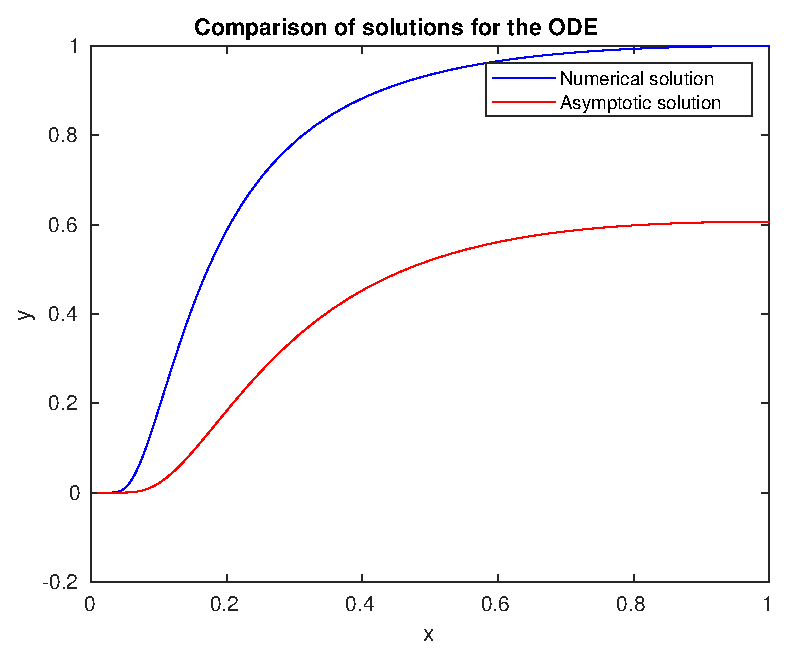
\includegraphics{TopicCA1Q2c}
        \end{figure}

    \end{enumerate}
%%%
%%Question 3
%%%

    \item 
    \begin{enumerate}
        \item 

        \begin{align*}
            S(\epsilon) &= \int_0^\infty \frac{e^{-t}}{1+\epsilon t} \,dt\\
            &= \int_0^\infty e^{-t} \left(\frac{(-\epsilon t)^{N+1}}{1+\epsilon t} + \sum_{j=0}^N (-\epsilon t)^j\right) \, dt\\
            &= \int_0^\infty e^{-t} \frac{(-\epsilon t)^{N+1}}{1+\epsilon t}\, dt + \int_0^\infty e^{-t} \sum_{j=0}^N (-\epsilon t)^j \, dt\\
            &= (-1)^{N+1}\epsilon^{N+1}\int_0^\infty  \frac{e^{-t}t^{N+1} }{1+\epsilon t}\, dt + \sum_{j=0}^N(-1)^j\epsilon^j\int_0^\infty e^{-t}   t^j \, dt\\
            &= (-1)^{N+1}\epsilon^{N+1}\int_0^\infty  \frac{e^{-t}t^{N+1} }{1+\epsilon t}\, dt + \sum_{j=0}^N(-1)^j\epsilon^j j!\\
            &= (-1)^{N+1}\epsilon^{N+1}\int_0^\infty  \frac{e^{-t}t^{N+1} }{1+\epsilon t}\, dt + \sum_{j=0}^N(-1)^j\epsilon^j j!\\
            &=\sum_{j=0}^N(-1)^j\epsilon^j j! + (-1)^{N+1}\epsilon^{N+1}\int_0^\infty  \frac{e^{-t}t^{N+1} }{1+\epsilon t}\, dt\\
            &= 1 - \epsilon + 2\epsilon^2 - 6\epsilon^3 + 24\epsilon^4 - \hdots  \\
            \end{align*}
            Using $\int_0^\infty e^{-x} x^{n} dx= n!$
            
            By truncating the series, at $N$, we get the error term as
            \[err(N) = (-1)^{N+1}\epsilon^{N+1}\int_0^\infty  \frac{e^{-t}t^{N+1} }{1+\epsilon t}\,dt\]
            
            It is optimal to truncate the series at the smallest term, i.e. the value of $j$ which gives the smallest value.
            So want the largest $j$ such that (and terminate the series before the $j+1$ term)
            \begin{align*}
                \epsilon^j j! \leq \epsilon^{j+1} (j+1)!\\
                1 \leq \epsilon (j+1)\\
                (j+1) \geq \frac{1}{\epsilon}\\
                j \geq \frac{1}{\epsilon} - 1
            \end{align*}
            
            
            
            
        \item  Using the error term
                    \[err(N) = (-1)^{N+1}\epsilon^{N+1}\int_0^\infty  \frac{e^{-t}t^{N+1} }{1+\epsilon t}\,dt\]
        And use 
        \[\frac{1}{1+\epsilon t} = \frac{1}{2[1 + \frac12 (\epsilon t - 1)]}\]
        \begin{align*}
            &err(N) = (-1)^{N+1}\epsilon^{N+1}\int_0^\infty  \frac{e^{-t}t^{N+1} }{1+\epsilon t}\,dt\\
            &=(-1)^{N+1}\epsilon^{N+1}\int_0^\infty  \left(e^{-t}t^{N+1}\right) \frac{1}{2[1 + \frac12 (\epsilon t - 1)]} \,dt\\
            &=(-1)^{N+1}\epsilon^{N+1}\frac12 \int_0^\infty  \left(e^{-t}t^{N+1}\right) \left( \left(\sum_{j=0}^{M} (-\frac12 (\epsilon t - 1))^j\right) + \frac{(-\frac12 (\epsilon t - 1))^{M+1}}{1 + \frac12 (\epsilon t - 1)}\right)\, dt\\
            &=(-1)^{N+1}\epsilon^{N+1}\frac12 \left(\int_0^\infty  \left(e^{-t}t^{N+1}\right) \sum_{j=0}^{M} (-\frac12 (\epsilon t - 1))^j\, dt + \int_0^\infty  \left(e^{-t}t^{N+1}\right)\frac{(-\frac12 (\epsilon t - 1))^{M+1}}{1 + \frac12 (\epsilon t - 1)}\, dt\right)\\
            &=(-1)^{N+1}\epsilon^{N+1}\frac12 \left( \sum_{j=0}^{M}\int_0^\infty  \left(e^{-t}t^{N+1}\right) (-\frac12)^j (\epsilon t - 1)^j\, dt + \int_0^\infty  \left(e^{-t}t^{N+1}\right)\frac{(-\frac12 (\epsilon t - 1))^{M+1}}{1 + \frac12 (\epsilon t - 1)}\, dt\right)\\
        \end{align*}
        Expanding the first $\sum\int$ term:
        \begin{align*}
            &\sum_{j=0}^{M}\int_0^\infty  \left(e^{-t}t^{N+1}\right) (-\frac12)^j (\epsilon t - 1)^j\, dt\\
            &=\sum_{j=0}^{M}(-\frac12)^j\int_0^\infty  \left(e^{-t}t^{N+1}\right) \sum_{k=0}^j \ncr{j}{k} (\epsilon t)^{k} (-1)^{j-k}\, dt\\
            &=\sum_{j=0}^{M}(-\frac12)^j \sum_{k=0}^j \ncr{j}{k}(-1)^{j-k} \int_0^\infty  \left(e^{-t}t^{N+1}\right)\epsilon^k t^{k} \, dt\\
            &=\sum_{j=0}^{M}(-\frac12)^j \sum_{k=0}^j \epsilon^k\ncr{j}{k}(-1)^{j-k} \int_0^\infty  \left(e^{-t}t^{N+k+1}\right)  \, dt\\
            &=\sum_{j=0}^{M}(-\frac12)^j \sum_{k=0}^j \epsilon^k\ncr{j}{k}(-1)^{j-k} (N+k+1)! \\
            &=\sum_{j=0}^{M}(\frac12)^j \sum_{k=0}^j \epsilon^k\ncr{j}{k}(-1)^{-k} (N+k+1)! \\
        \end{align*}
        So it gives
        
        \[err(N) = (-1)^{N+1}\epsilon^{N+1}\frac12 \left( \sum_{j=0}^{M}(\frac12)^j \sum_{k=0}^j \epsilon^k\ncr{j}{k}(-1)^{-k} (N+k+1)!\right) + errerr(N,M)\]

        Where
        \begin{align*}
            errerr(N,M) = (-1)^{N+1}\epsilon^{N+1}\frac12 \left(\int_0^\infty  \left(e^{-t}t^{N+1}\right)\frac{(-\frac12 (\epsilon t - 1))^{M+1}}{1 + \frac12 (\epsilon t - 1)}\, dt\right)\\
            errerr(N,M) = (-1)^{N+M+2}\epsilon^{N+1}\left(\frac12\right)^{M+2} \left(\int_0^\infty  \left(e^{-t}t^{N+1}\right)\frac{ (\epsilon t - 1)^{M+1}}{1 + \frac12 (\epsilon t - 1)}\, dt\right)  
        \end{align*}
        
        \item Figure~\ref{fig:3c1} shows the absolute error obtained in (a), while figure~\ref{fig:3c2} shows the error, ``errerr'' obtained in (b), both for an epsilon value of $\epsilon = 0.1$. The optimal truncation for the first series (denoted by the red cross in figure~\ref{fig:3c1}) occurs for $N=9$.
        From figure~\ref{fig:3c2}, the optimal truncation point shifts 


        \begin{figure}
        \centering
        \label{fig:3c1}
        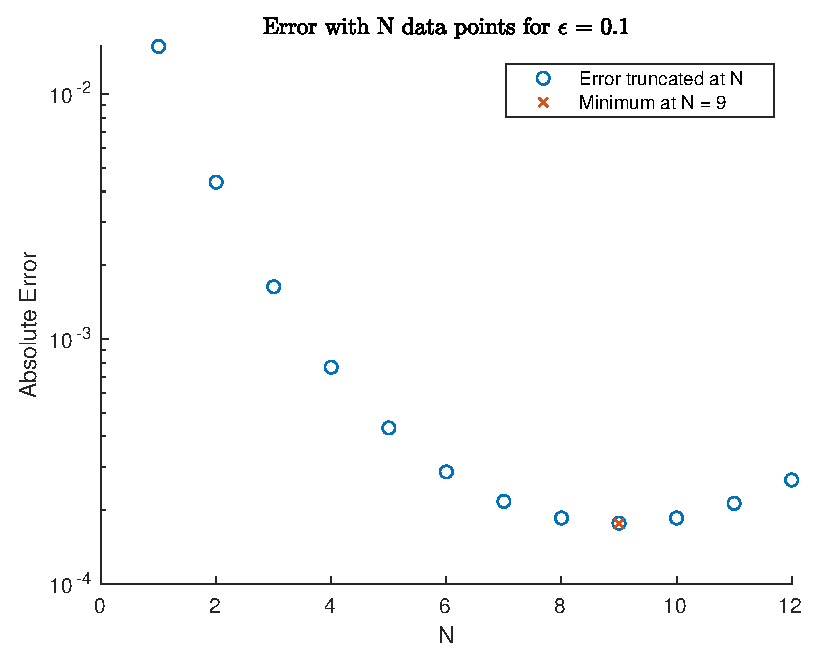
\includegraphics{TopicCA1Q3c1}
        \caption{Plot of the absolute error term against $N$ on a log y scale}
        \end{figure}
        \begin{figure}
        \centering
        \label{fig:3c2}
        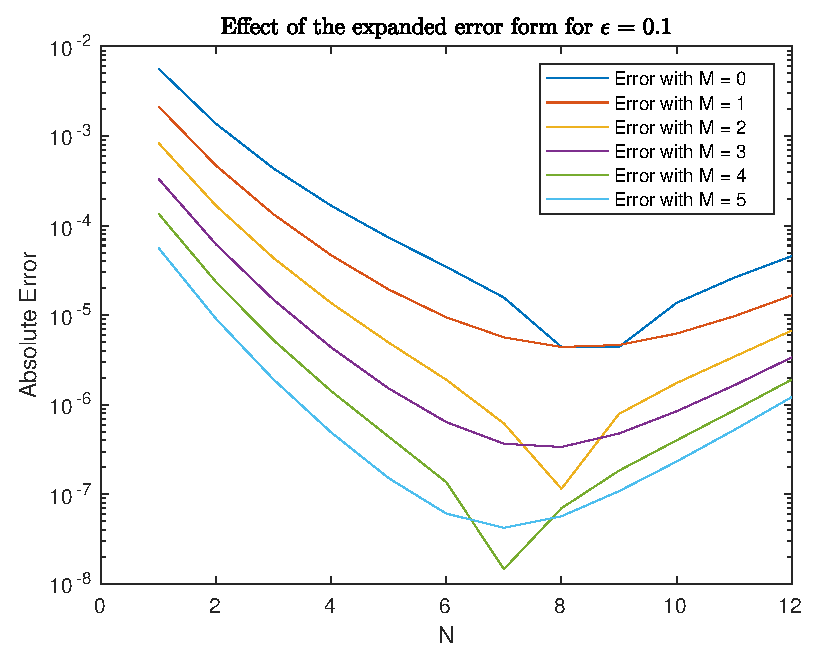
\includegraphics{TopicCA1Q3c2}
        \caption{Plot of the second absolute error term (``errerr'') for various $M$ on a log y scale}
        \end{figure}
    \end{enumerate}
\end{enumerate}

\clearpage

\section*{Matlab Code}
\lstinputlisting{AppTopicCA1.m}


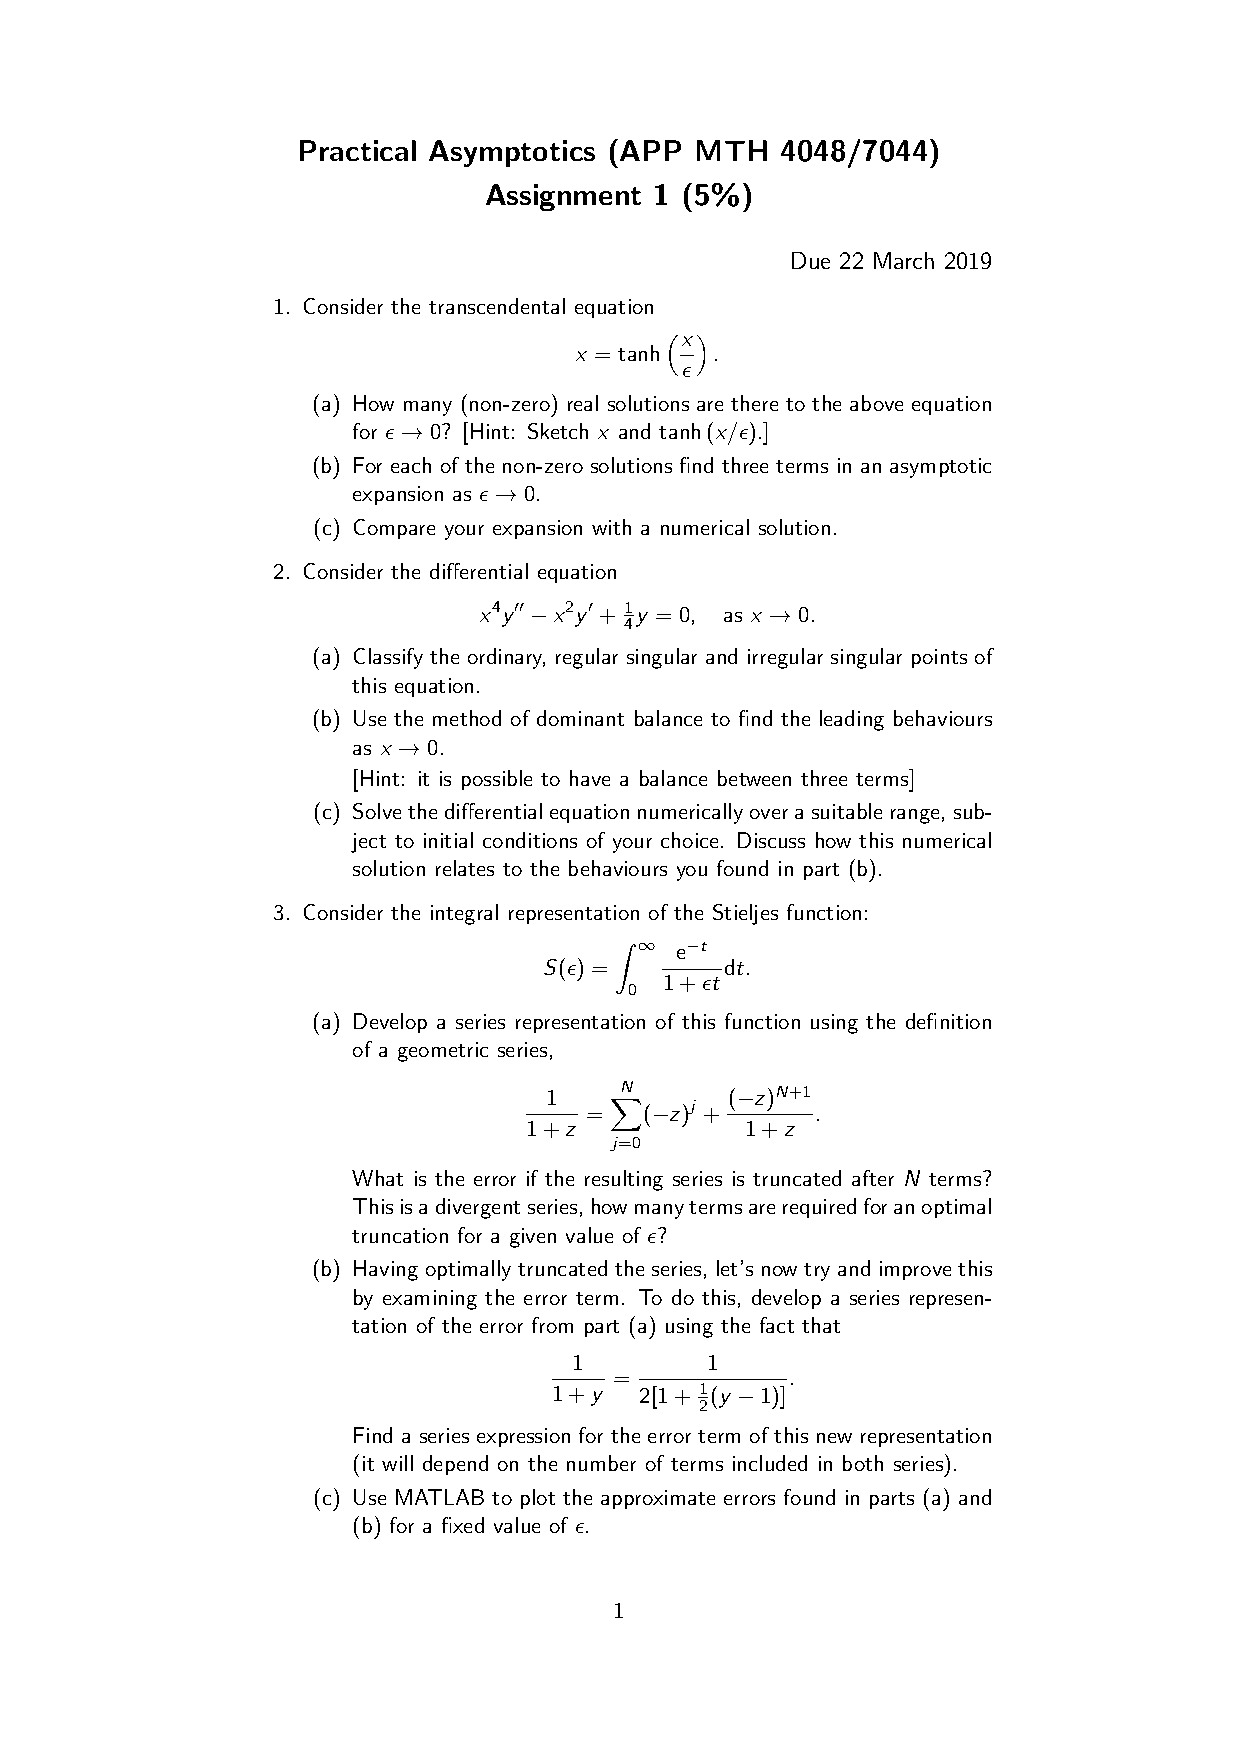
\includepdf[pages=1-]{PA_2019_A1.pdf}

\end{document}
